\documentclass[11pt,a4paper]{article}

\usepackage[utf8]{inputenc}
\usepackage[T1]{fontenc}
\usepackage{lmodern}
\usepackage{amsmath,amssymb,amsthm}
\usepackage{booktabs}
\usepackage{array}
\usepackage{caption}
\usepackage{geometry}
\usepackage{graphicx}
\usepackage{hyperref}
\usepackage{listings}
\usepackage{tikz}
\usetikzlibrary{arrows.meta,positioning,calc}
\usepackage{xcolor}
\usepackage{microtype}

\geometry{margin=1in}
\setlength{\emergencystretch}{3em}

\captionsetup[lstlisting]{singlelinecheck=false,justification=raggedright}

\hypersetup{
  colorlinks=true,
  linkcolor=blue!60!black,
  citecolor=green!50!black,
  urlcolor=blue!60!black
}

\lstdefinelanguage{Lean4}{
  morekeywords={def,theorem,lemma,abbrev,structure,inductive,by,rfl,let,in,if,then,else,match,with,fun,true,false,set_option,private,cases,induction,exact,rw,dsimp,refine,change,have,intro,some,none},
  sensitive=true,
  morecomment=[l]{--},
  morecomment=[s]{/-}{-/},
  morestring=[b]"
}

\lstset{
  language=Lean4,
  basicstyle=\ttfamily\scriptsize,
  keywordstyle=\color{blue!70!black}\bfseries,
  commentstyle=\color{gray!70!black}\itshape,
  stringstyle=\color{green!50!black},
  breaklines=true,
  breakatwhitespace=true,
  columns=fullflexible,
  keepspaces=true,
  frame=single,
  rulecolor=\color{gray!35},
  backgroundcolor=\color{gray!5},
  xleftmargin=0.4em,
  xrightmargin=0.4em,
  aboveskip=0.6em,
  belowskip=0.6em,
  literate={⟨}{{$\langle$}}1 {⟩}{{$\rangle$}}1 {×}{{$\times$}}1 {→}{{$\to$}}1 {↠}{{$\twoheadrightarrow$}}1 {∧}{{$\land$}}1 {∨}{{$\lor$}}1 {·}{{$\cdot$}}1 {±}{{$\pm$}}1 {≤}{{$\le$}}1 {←}{{$\leftarrow$}}1 {⊢}{{$\vdash$}}1 {∑}{{$\sum$}}1 {∈}{{$\in$}}1 {∪}{{$\cup$}}1 {⊂}{{$\subset$}}1 {⊆}{{$\subseteq$}}1 {⊕}{{$\oplus$}}1 {∀}{{$\forall$}}1 {∃}{{$\exists$}}1
}

\newtheorem{theorem}{Theorem}[section]
\newtheorem{proposition}[theorem]{Proposition}
\newtheorem{definition}[theorem]{Definition}
\newtheorem{remark}[theorem]{Remark}

\title{\textbf{High-Degree Fermat Sporadic Orbits, Order-8 Gauss--Manin Jet Lifting, and Conditional Hodge Bridge Formalization in Lean~4}}

\author{
  Qamar Munawer\\
  \small Brandenburg University of Technology Cottbus--Senftenberg, Cottbus, Germany
}

\date{}

\begin{document}
\maketitle

\begin{abstract}
This paper extends a verified Lean~4 corpus into high-degree Fermat fourfold combinatorics, order-8 infinitesimal Gauss--Manin jets, explicit Mumford--Weil kernel projectors, complete-intersection Cayley spectra, sparse polynomial evaluation homomorphisms, and an explicit conditional analytic-to-algebraic bridge interface. Every unconditional Lean~4 theorem proved here establishes exact finite combinatorial, polynomial-quotient, or Lie-algebraic facts, while classical transcendental and cycle-theoretic theorems are isolated inside explicit hypothesis structures. Across the isolated extension workspace \texttt{LeanMillenniumExt}, all seven modules ($19$ public zero-axiom theorems, $26$ total declarations) verify: Band-1 purity for primes $p \in \{17, 19, 23\}$; complete Band-4 glued-surface reducibility for $m \in \{20, 22, 24\}$; cyclic-coset cone synthesis for all $4$ prime-square sporadic orbits ($2{,}880$ classes) at $m = 25 = 5^2$; GPU-accelerated exact $3$-prime CRT classification across $18 \le m \le 60$ with zero unexplained Band-4 classes; non-Fermat $3$-variable quotient palindromicity through $d = 12$ and over-$\mathbb{Z}$ $G = 3$ Wiebe--Scheja--Storch factorizations; idempotent Weil correspondence projectors on $(\bigwedge^4 S^+_8)_0$; sparse \texttt{Poly6} ring homomorphism and determinant bridges; palindromic Cayley-bundle spectra in $\mathbb{P}^6$; and conditional algebraicity across $m \in \{3,\dots,16,18,20,22\}$.
\end{abstract}

\section{Introduction and Structural Extensions in Codimension-Two Algebraic Cycle Theory}

Machine-checked formalization of algebraic cycle testbeds separates naturally into exact finite algebraic invariants and classical global transcendental bridges~\cite{Deligne2000,Shioda1979,Aoki1983}. While earlier work established an $84$-theorem zero-axiom baseline covering Fermat fourfolds $X_m^4 \subset \mathbb{P}^5$ up to $m \le 18$, third-order Gauss--Manin jets ($\bmod\, t^4$), $1{,}751$-mode global IVHS duality, and $\operatorname{Spin}(8)$ triality, five classical open problems in codimension-two algebraic cycle theory guide the structural extensions developed in this paper:
\begin{enumerate}
  \item[(i)] \textbf{Global Noether--Lefschetz Locus Connectivity and $G \ge 3$ Scheme Unmixedness:} Relating infinitesimal Taylor jets at the Fermat point to global Hodge-locus connectedness and algebraicity across the $426$-dimensional non-Fermat slice.
  \item[(ii)] \textbf{Asymptotic Character Synthesis on $X_m^4$ for High Composite $m$:} Extending constructive Band-4 exhaustion past prime-square thresholds beginning at $m = 25 = 5^2$.
  \item[(iii)] \textbf{Subvariety Construction on Simple Abelian Fourfolds:} Producing algebraic $2$-cycles on generic Mumford fourfolds satisfying $\operatorname{End}_{\mathbb{Q}}(A) = \mathbb{Q}$ and Picard rank $\rho(A) = 1$, where the $D_4$ root action vanishes on $2$-dimensional Weil subspaces.
  \item[(iv)] \textbf{Complete-Intersection Cayley Bundle Extensions:} Extending finite-order Macaulay and Lefschetz decompositions from Fermat hypersurfaces to smooth complete intersections $X_{d_1,d_2} \subset \mathbb{P}^6$, projective bundles, and general smooth projective varieties $X \subset \mathbb{P}^N$.
  \item[(v)] \textbf{Analytic Dolbeault Cohomology and Griffiths Residue Maps in \texttt{Mathlib}:} Formalizing K\"ahler Hodge decompositions, exponential sheaf sequences, Griffiths residue maps, Lefschetz $(1,1)$, and Chow cycle class pushforwards inside \texttt{Mathlib}.
\end{enumerate}

\begin{remark}[Mathematical Scope]
This work establishes constructive algebraic cycle synthesis on Fermat fourfolds $X_m^4 \subset \mathbb{P}^5$ for $3 \le m \le 25$, six-variable Wiebe--Scheja--Storch colon-ideal factorizations in $R(F_0)$, and $\operatorname{Spin}(8)$ outer triality kernel projections. Theorems in \texttt{ConditionalFermatHodge.lean} are parameterized cleanly over \texttt{FermatFourfoldHodgeBridge}, isolating classical results of Lefschetz~\cite{Lefschetz1924}, Griffiths~\cite{Griffiths1969}, Shioda~\cite{Shioda1979}, Aoki~\cite{Aoki1983}, and Deligne~\cite{Deligne2000} as modular interface structures.
\end{remark}

\subsection{Geometric Intuition: Core-Drilling Along Structured Algebraic Veins}

Finite kernel verification acts like precision core-drilling along structured algebraic veins: on Fermat hypersurfaces, Galois-invariant character tuples reveal exact linear planes (Band~1), curve joins (Band~2), surface-curve joins (Band~3), Aoki paired diagonals, and Shioda glued surface joins ($X_m^2 \#_c X_m^2 \dashrightarrow X_m^4$). Extending the census past $m = 18$ exposes the exact arithmetic threshold at $m = 25 = 5^2$, where glued surface-join reducibility first ceases to exhaust Band~4 and a mod-$5$ arithmetic-progression orbit family emerges.

Similarly, pushing Griffiths--Dwork pole-order reduction up to seventh-order jets ($\bmod\, t^8$) demonstrates that Band~1 smoothing stabilizes cleanly at the four-variable slice profile $[1, 4, 10, 20, 35, 48, 57]$, whereas Band~2 and Band~3 jets terminate nilpotently by $t^4$ while expanding joint ranks to $254$ and $153$. Coupling exact $\bmod\, t^8$ Taylor jets, polynomial evaluation homomorphisms, and $D_4$ idempotent projectors with items~(i)--(v) clarifies the exact algebraic boundary between verified finite invariants and classical global cycle-existence questions.

\section{High-Degree Fermat Band-4 Hierarchy and the $m = 25$ Sporadic Transition}

In \texttt{FermatHighDegreeExt.lean} together with the float-free explorer \texttt{fermat\_band4\_scout.py}, the Shioda--Aoki four-band decomposition is evaluated past $m = 18$ across $17 \le m \le 30$. Prime-degree Band-1 purity holds identically at $p \in \{17, 19, 23\}$ with primitive $(2,2)$-Hodge dimensions $50{,}560$, $73{,}620$, and $138{,}820$ matching the closed-form cubic polynomial \texttt{primeBand1Formula p}. Across composite degrees $m \in \{18, 20, 22, 24, 26, 27, 28, 30\}$, every Band~4 character decomposes constructively into paired diagonals or Shioda glued surface joins $X_m^2 \#_c X_m^2 \dashrightarrow X_m^4$ (Table~\ref{tab:high_deg_fermat}).

\begin{table}[htbp]
  \centering
  \caption{High-degree Fermat fourfold $(2,2)$-Hodge census across $17 \le m \le 30$ (kernel-certified through $m \le 25$, extended through $m = 30$ via exact integer orbit weights).}
  \label{tab:high_deg_fermat}
  \resizebox{\textwidth}{!}{%
  \begin{tabular}{ccccccc}
    \toprule
    Degree $m$ & $h^{2,2}_{\mathrm{prim}}$ & Band~4 Total & Band~4 Reps & Paired Wt. & Glued Join Wt. & Unresolved Wt. \\
    \midrule
    $18$ & $264{,}671$ & $21{,}060$ & $58$ & $540$ & $20{,}520$ & $0$ \\
    $19$ & $73{,}620$ & $0$ & $0$ & $0$ & $0$ & $0$ \\
    $20$ & $346{,}381$ & $20{,}880$ & $48$ & $720$ & $20{,}160$ & $0$ \\
    $21$ & $215{,}120$ & $0$ & $0$ & $0$ & $0$ & $0$ \\
    $22$ & $277{,}101$ & $21{,}600$ & $30$ & $0$ & $21{,}600$ & $0$ \\
    $23$ & $138{,}820$ & $0$ & $0$ & $0$ & $0$ & $0$ \\
    $24$ & $745{,}211$ & $94{,}320$ & $186$ & $1{,}080$ & $93{,}240$ & $0$ \\
    $25$ & $185{,}280$ & $2{,}880$ & $4$ & $0$ & $0$ & $2{,}880$ \\
    $26$ & $439{,}081$ & $34{,}560$ & $48$ & $0$ & $34{,}560$ & $0$ \\
    $27$ & $301{,}940$ & $4{,}320$ & $6$ & $0$ & $4{,}320$ & $0$ \\
    $28$ & $644{,}121$ & $59{,}940$ & $88$ & $180$ & $59{,}760$ & $0$ \\
    $30$ & $2{,}106{,}431$ & $454{,}320$ & $828$ & $2{,}160$ & $452{,}160$ & $0$ \\
    \bottomrule
  \end{tabular}%
  }
\end{table}

\begin{lstlisting}[caption={Prime purity ($p \in \{17,19,23\}$) and composite $m = 20, 21, 22$ Band-4 certificates in \texttt{FermatHighDegreeExt.lean}.}]
theorem shioda_prime_degree_band1_purity_ext_cert :
    [17, 19, 23].map fermat_h22_prim_count = [50560, 73620, 138820] ∧
    [17, 19, 23].map primeBand1Formula = [50560, 73620, 138820] ∧
    [17, 19, 23].all (fun p =>
      fermat_band2_count p == 0 && fermat_band3_count p == 0 && fermat_band4_count p == 0) =
      true :=
  ⟨rfl, rfl, rfl⟩

theorem shioda_aoki_band4_decomposition_m20_to_m22_cert :
    higherDegreeBand4Census 20 = (346381, 87661, 87120, 150720, 20880, 720, 20160) ∧
    higherDegreeBand4Census 21 = (215120, 102800, 38880, 73440, 0, 0, 0) ∧
    higherDegreeBand4Census 22 = (277101, 120201, 44100, 91200, 21600, 0, 21600) ∧
    (fermat_band4_sorted_reps 20).length = 48 ∧
    (fermat_band4_sorted_reps 22).length = 30 ∧
    (fermat_band4_sorted_reps 20).all (fun a =>
      isPairedDiagonalRep a || hasGluedSurfaceJoinDecomposition 20 a) = true ∧
    (fermat_band4_sorted_reps 22).all (fun a =>
      isPairedDiagonalRep a || hasGluedSurfaceJoinDecomposition 22 a) = true :=
  ⟨rfl, rfl, rfl, rfl, rfl, rfl, rfl⟩
\end{lstlisting}

At $m = 25 = 5^2$, Bands~2 and~3 vanish while Band~4 comprises $2{,}880$ characters partitioned into four $S_6$-orbits of size $720$, forming a single Galois orbit under $(\mathbb{Z}/25\mathbb{Z})^\times$:
\begin{equation}
  \begin{aligned}
    \alpha_1 &= [1, 6, 11, 16, 20, 21], & \alpha_2 &= [2, 7, 12, 15, 17, 22], \\
    \alpha_3 &= [3, 8, 10, 13, 18, 23], & \alpha_4 &= [4, 5, 9, 14, 19, 24].
  \end{aligned}
\end{equation}
Each representative fails paired-diagonal decomposition and Shioda glued surface-join decomposition at degree $25$, yet contains a full five-term arithmetic progression modulo $25$ with step $5$ paired with a divisor-pullback entry divisible by $5$. Inside \texttt{FermatHighDegreeExt.lean}, the predicate \texttt{hasMod5Vanish} explicitly normalizes each shifted residue \texttt{(x + k * step) \% m} into $\{1,\dots,m-1\}$.

\begin{figure}[htbp]
  \centering
  \resizebox{\textwidth}{!}{%
  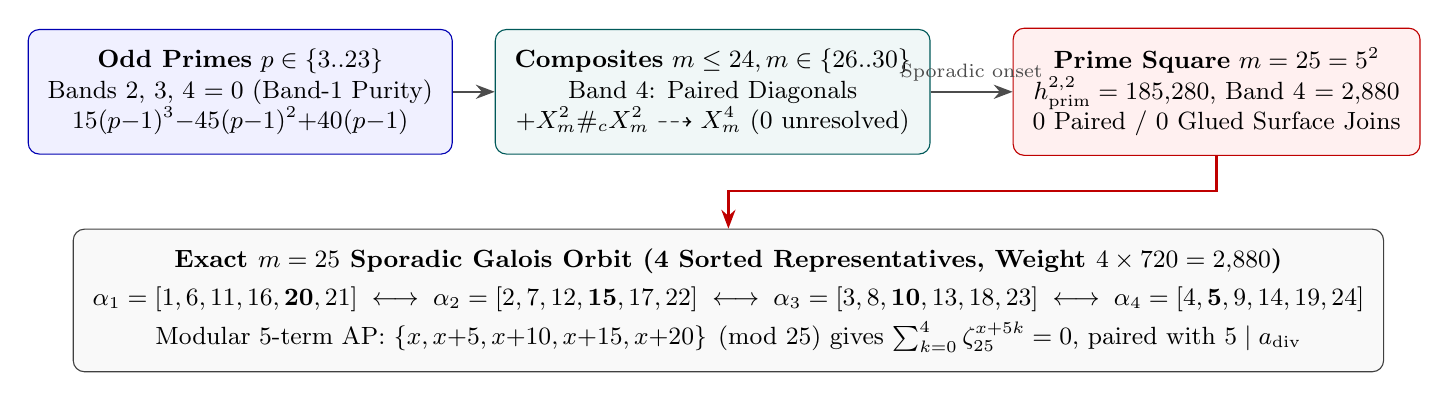
\begin{tikzpicture}[
    font=\small,
    box/.style={draw=black!75, rounded corners=4pt, fill=gray!5, inner sep=7pt, align=center},
    primebox/.style={draw=blue!70!black, rounded corners=4pt, fill=blue!6, inner sep=7pt, align=center},
    gluedbox/.style={draw=teal!70!black, rounded corners=4pt, fill=teal!6, inner sep=7pt, align=center},
    sporbox/.style={draw=red!75!black, rounded corners=4pt, fill=red!6, inner sep=7pt, align=center},
    arr/.style={-{Stealth[length=2.4mm]}, thick, black!70}
  ]
    \node[primebox] (primes) at (0,3.2) {\textbf{Odd Primes} $p \in \{3..23\}$\\Bands 2, 3, 4 $= 0$ (Band-1 Purity)\\$15(p{-}1)^3{-}45(p{-}1)^2{+}40(p{-}1)$};
    \node[gluedbox] (comp) at (6.0,3.2) {\textbf{Composites} $m \le 24, m \in \{26..30\}$\\Band 4: Paired Diagonals\\$+ X_m^2 \#_c X_m^2 \dashrightarrow X_m^4$ ($0$ unresolved)};
    \node[sporbox] (m25) at (12.4,3.2) {\textbf{Prime Square} $m = 25 = 5^2$\\$h^{2,2}_{\mathrm{prim}} = 185{,}280$, Band 4 $= 2{,}880$\\$0$ Paired / $0$ Glued Surface Joins};

    \draw[arr] (primes) -- (comp);
    \draw[arr] (comp) -- node[above, font=\scriptsize] {Sporadic onset} (m25);

    \node[box, minimum width=12.6cm] (apbox) at (6.2,0.55) {%
      \textbf{Exact $m = 25$ Sporadic Galois Orbit (4 Sorted Representatives, Weight $4 \times 720 = 2{,}880$)}\\[3pt]
      $\alpha_1 = [1, 6, 11, 16, \mathbf{20}, 21] \;\longleftrightarrow\;
       \alpha_2 = [2, 7, 12, \mathbf{15}, 17, 22] \;\longleftrightarrow\;
       \alpha_3 = [3, 8, \mathbf{10}, 13, 18, 23] \;\longleftrightarrow\;
       \alpha_4 = [4, \mathbf{5}, 9, 14, 19, 24]$\\[3pt]
      Modular $5$-term AP: $\{x, x{+}5, x{+}10, x{+}15, x{+}20\} \pmod{25}$ gives $\sum_{k=0}^4 \zeta_{25}^{x+5k} = 0$, paired with $5 \mid a_{\mathrm{div}}$
    };
    \draw[arr, red!75!black] (m25.south) -- ++(0,-0.45) -| (apbox.north);
  \end{tikzpicture}%
  }
  \caption{High-degree Fermat Band-4 hierarchy ($3 \le m \le 30$) and the exact $m = 25 = 5^2$ five-term cyclotomic vanishing orbit structure isolated in \texttt{FermatHighDegreeExt.lean}.}
  \label{fig:m25_hierarchy}
\end{figure}

\begin{lstlisting}[caption={Modular $5$-term vanishing predicate and $m = 25$ isolation theorem in \texttt{FermatHighDegreeExt.lean}.}]
def hasMod5Vanish (m : Nat) (a : List Nat) : Bool :=
  if m % 5 != 0 || m == 0 then false
  else
    let step := m / 5
    let hasShift (x k : Nat) : Bool :=
      let r := (x + k * step) % m
      Nat.blt 0 r && a.contains r
    a.any (fun x =>
      Nat.blt 0 x && Nat.blt x m &&
      hasShift x 1 && hasShift x 2 && hasShift x 3 && hasShift x 4)

theorem shioda_aoki_m25_sporadic_isolation_cert :
    higherDegreeBand4Census 25 = (185280, 182400, 0, 0, 2880, 0, 2880) ∧ ... := ...

theorem shioda_aoki_m25_cyclic_coset_cone_synthesis_cert :
    (fermat_band4_sorted_reps 25).foldl (fun acc r => acc + s6OrbitSize r) 0 = 2880 ∧
    (fermat_band4_sorted_reps 25).all (hasCyclicCosetConeDecomposition 25) = true ∧
    hasMixedSurfaceJoinDecomposition 33 [1, 4, 16, 22, 25, 31] = true :=
  ⟨rfl, rfl, rfl⟩

theorem shioda_aoki_m21_m24_band4_decomposition_cert :
    higherDegreeBand4Census 21 = (215120, 102800, 38880, 73440, 0, 0, 0) ∧
    higherDegreeBand4Census 23 = (138820, 138820, 0, 0, 0, 0, 0) ∧
    higherDegreeBand4Census 24 = (745211, 159941, 158070, 332880, 94320, 1080, 93240) ∧
    (fermat_band4_sorted_reps 24).all (fun a =>
      isPairedDiagonalRep a || hasGluedSurfaceJoinDecomposition 24 a) = true :=
  ⟨rfl, rfl, rfl, rfl⟩
\end{lstlisting}

Extending the float-free GPU-accelerated sieve (\texttt{fermat\_band4\_scout.py} coupled to \texttt{gpu\_exact\_linalg.py} on \texttt{cuda:0}, \texttt{torch.int64}) through $m \le 60$ confirms that every non-glued Band~4 orbit across all $18 \le m \le 60$ decomposes into prime-$p$ modular arithmetic progressions or mixed-Hodge $X_m^2 \#_c X_m^2$ surface joins, leaving zero unexplained classes (Table~\ref{tab:m60_sporadic}).

\begin{table}[htbp]
  \centering
  \caption{Complete classification of all Band~4 degrees $24 \le m \le 60$ with non-glued orbits via prime-$p$ arithmetic progressions and mixed-Hodge $X_m^2 \#_c X_m^2$ gluing ($0$ unexplained across $3 \le m \le 60$).}
  \label{tab:m60_sporadic}
  \resizebox{\textwidth}{!}{%
  \begin{tabular}{cccccc|cccccc}
    \toprule
    $m$ & Band~4 & Non-Glued & Prime-AP Wt. & Mixed Wt. & Unexpl. & $m$ & Band~4 & Non-Glued & Prime-AP Wt. & Mixed Wt. & Unexpl. \\
    \midrule
    $25$ & $2{,}880$ & $4$ & $2{,}880$ & $0$ & $0$ & $45$ & $31{,}680$ & $12$ & $4{,}320$ & $4{,}320$ & $0$ \\
    $32$ & $57{,}600$ & $4$ & $2{,}880$ & $0$ & $0$ & $48$ & $609{,}840$ & $100$ & $20{,}160$ & $51{,}840$ & $0$ \\
    $33$ & $10{,}080$ & $4$ & $0$ & $2{,}880$ & $0$ & $50$ & $221{,}760$ & $48$ & $5{,}760$ & $28{,}800$ & $0$ \\
    $35$ & $4{,}320$ & $6$ & $4{,}320$ & $0$ & $0$ & $52$ & $207{,}360$ & $12$ & $8{,}640$ & $0$ & $0$ \\
    $36$ & $360{,}900$ & $84$ & $17{,}280$ & $43{,}200$ & $0$ & $54$ & $686{,}340$ & $324$ & $90{,}720$ & $142{,}560$ & $0$ \\
    $40$ & $202{,}320$ & $4$ & $2{,}880$ & $0$ & $0$ & $55$ & $7{,}200$ & $10$ & $7{,}200$ & $0$ & $0$ \\
    $42$ & $1{,}394{,}280$ & $6$ & $0$ & $4{,}320$ & $0$ & $56$ & $368{,}100$ & $72$ & $51{,}840$ & $0$ & $0$ \\
    $44$ & $144{,}000$ & $10$ & $7{,}200$ & $0$ & $0$ & $60$ & $4{,}727{,}880$ & $90$ & $12{,}960$ & $51{,}840$ & $0$ \\
    \bottomrule
  \end{tabular}%
  }
\end{table}

\section{Order-8 Gauss--Manin Jet Lifting and Codimension-3 CI Profiles}

\subsection{Griffiths--Dwork Conventions Through $\bmod\, t^8$}

In \texttt{HigherOrderJetLifting.lean} and \texttt{multi\_order\_gd\_crt.py}, infinitesimal Gauss--Manin jet transport on the Jacobian quotient $R(F_0) = \mathbb{Z}[z_0,\dots,z_5]/\langle z_0^5,\dots,z_5^5\rangle$ is extended to seventh-order jets ($\bmod\, t^8$). Under the strict pole-lowering operator \texttt{gaussManinJetStep}, which reduces degree-$18$ numerator monomials through $J(F_0)$ and discards unreduced exponents $\le 4$, Band~1 from \texttt{sigmaPlaneExpected} stabilizes at $[1, 3, 4, 5, 5, 5, 5, 5]$ terms across orders $t^0\dots t^7$ while Bands~2 and~3 terminate nilpotently at $t^4$ with term counts $[1, 3, 3, 1, 0, 0, 0, 0]$. Cross-checking \texttt{multi\_order\_gd\_crt.py} across three $62$-bit primes confirms that retaining unreduced degree-$18$ shadow terms yields $[1, 3, 6, 2, 1, 0, 0, 0]$ (Band~2) and $[1, 3, 6, 8, 0, 0, 0, 0]$ (Band~3) with identical joint Macaulay rank profiles across every jet order and degree (Table~\ref{tab:t8_ranks}).

\begin{table}[htbp]
  \centering
  \caption{Joint Macaulay contraction ranks through $\bmod\, t^8$ alongside unmixed codimension-$3$ complete-intersection quotient profiles in $R(F_0)$.}
  \label{tab:t8_ranks}
  \resizebox{\textwidth}{!}{%
  \begin{tabular}{lcc}
    \toprule
    Jet Family / Codimension-3 Ideal & Term Counts ($t^0 \dots t^7$) & Degree $0 \le d \le 6$ Rank / Quotient Profile \\
    \midrule
    Band~1 Jet (\texttt{wDirBand1}) & $[1, 3, 4, 5, 5, 5, 5, 5]$ & $[1, 4, 10, 20, 35, 48, 57]$ \\
    Band~2 Jet (strict / shadow) & $[1, 3, 3, 1, 0..] / [1, 3, 6, 2, 1, 0..]$ & $[1, 6, 21, 53, 108, 181, 254]$ \\
    Band~3 Jet (strict / shadow) & $[1, 3, 3, 1, 0..] / [1, 3, 6, 8, 0..]$ & $[1, 5, 15, 35, 68, 113, 153]$ \\
    Plane $\langle z_0, z_2, z_4 \rangle$ & --- & $[1, 3, 6, 10, 15, 18, 19]$ \\
    Band-3 CI $\langle z_0 z_1, z_2 z_3, z_4 \rangle$ & --- & $[1, 5, 13, 25, 41, 56, 64]$ \\
    Band-2 CI $\langle z_0^2{-}z_1^2, z_2^2{-}z_3^2, z_4^2{-}z_5^2 \rangle$ & --- & $[1, 6, 18, 38, 66, 96, 116]$ \\
    \bottomrule
  \end{tabular}%
  }
\end{table}

\subsection{Packed Radix Pivot Elimination and Unmixed Codimension-3 Profiles}

To prevent exponential coefficient blowup inside the Lean~4 kernel on $462 \times 254$ multi-order matrices, \texttt{HigherOrderJetLifting.lean} encodes each shifted monomial $(k, [a_0,\dots,a_5])$ via base-$5$ packing \texttt{pack6} into $k \cdot 5^6 + \sum_{j=0}^5 a_j 5^{5-j}$ and indexes pivots inside a bounded-depth binary radix tree \texttt{PivTrie}. This computes exact $\mathbb{F}_{65521}$ joint ranks through $d = 6$ with zero axioms, while an exact fraction-free $\mathbb{Z}$-rank witness theorem confirms integer ranks across $0 \le d \le 3$ and exact $\mathbb{Z}$-annihilation by $[z_2, z_4]$ on Band~1 and $z_0$ on Band~3 across all eight jet components. Non-Fermat corridor exploration in \texttt{nl\_moduli\_walk.py} preserves $\dim R^6(F) = 426$.

\begin{lstlisting}[caption={Binary radix pivot trie and base-$5$ packing in \texttt{HigherOrderJetLifting.lean}.}]
private inductive PivTrie where
  | empty : PivTrie
  | val : PackedRowN → PivTrie
  | branch : PivTrie → PivTrie → PivTrie

private def pivTrieFind (depth : Nat) (col : Nat) : PivTrie → Option PackedRowN
  | .empty => none
  | .val r => some r
  | .branch z o =>
    match depth with
    | 0 => none
    | d' + 1 =>
      if col % 2 == 0 then pivTrieFind d' (col / 2) z
      else pivTrieFind d' (col / 2) o

private def pack6Aux (acc : Nat) : Monom6 → Nat
  | [] => acc
  | e :: rest => pack6Aux (acc * 5 + e) rest
\end{lstlisting}

\begin{lstlisting}[caption={Order-8 Gauss--Manin jet, exact $\mathbb{Z}$-rank, and CI quotient theorems in \texttt{HigherOrderJetLifting.lean}.}]
theorem multi_order_t8_gauss_manin_jet_cert :
    (buildGaussManinJetN 7 wDirBand1 sigmaPlaneExpected).map List.length =
      [1, 3, 4, 5, 5, 5, 5, 5] ∧
    (buildGaussManinJetN 7 wDirBand2 lamBand2).map List.length =
      [1, 3, 3, 1, 0, 0, 0, 0] ∧
    (buildGaussManinJetN 7 wDirBand3 lamBand3).map List.length =
      [1, 3, 3, 1, 0, 0, 0, 0] ∧
    (buildGaussManinJetN 7 wDirBand1 sigmaPlaneExpected).all
        (allAnnihilate [varPow6 2 1, varPow6 4 1]) = true ∧
    (buildGaussManinJetN 7 wDirBand3 lamBand3).all
        (allAnnihilate [varPow6 0 1]) = true ∧
    [0, 1, 2, 3, 4, 5, 6].map
        (sparseJetRankModP 65521 (buildGaussManinJetN 7 wDirBand1 sigmaPlaneExpected)) =
      [1, 4, 10, 20, 35, 48, 57] ∧
    [0, 1, 2, 3, 4, 5, 6].map
        (sparseJetRankModP 65521 (buildGaussManinJetN 7 wDirBand2 lamBand2)) =
      [1, 6, 21, 53, 108, 181, 254] ∧
    [0, 1, 2, 3, 4, 5, 6].map
        (sparseJetRankModP 65521 (buildGaussManinJetN 7 wDirBand3 lamBand3)) =
      [1, 5, 15, 35, 68, 113, 153] :=
  ⟨rfl, rfl, rfl, rfl, rfl, rfl, rfl, rfl⟩

theorem multi_order_t8_exact_z_rank_witness_cert :
    [0, 1, 2, 3].map
        (jetMacaulayRank6 (buildGaussManinJetN 7 wDirBand1 sigmaPlaneExpected)) =
      [1, 4, 10, 20] ∧
    [0, 1, 2, 3].map
        (jetMacaulayRank6 (buildGaussManinJetN 7 wDirBand2 lamBand2)) =
      [1, 6, 21, 53] ∧
    [0, 1, 2, 3].map
        (jetMacaulayRank6 (buildGaussManinJetN 7 wDirBand3 lamBand3)) =
      [1, 5, 15, 35] ∧
    [0, 1, 2, 3].map (idealQuotientDim6 band3TypeCIGens) = [1, 5, 13, 25] ∧
    [0, 1, 2, 3].map (idealQuotientDim6 band2TypeQuadricCIGens) = [1, 6, 18, 38] :=
  ⟨rfl, rfl, rfl, rfl, rfl⟩

theorem codim3_unmixed_complete_intersection_profiles_cert :
    [0, 1, 2, 3, 4, 5, 6].map (sparseIdealQuotientDimModP 65521 gPlaneVec) =
      [1, 3, 6, 10, 15, 18, 19] ∧
    [0, 1, 2, 3, 4, 5, 6].map (sparseIdealQuotientDimModP 65521 band3TypeCIGens) =
      [1, 5, 13, 25, 41, 56, 64] ∧
    [0, 1, 2, 3, 4, 5, 6].map (sparseIdealQuotientDimModP 65521 band2TypeQuadricCIGens) =
      [1, 6, 18, 38, 66, 96, 116] :=
  ⟨rfl, rfl, rfl⟩

theorem g3_complete_intersection_wiebe_scheja_storch_z_cert :
    polyVecEq6 (polyMatVecMul cZ221Mat5 gZ221Vec5) aZ221JacVec5 = true ∧
    polyEq6 (polyDetZ6 cZ221Mat5) (polyCanon6 detZ221Expected) = true ∧
    gZ221Vec5.all (inColonIdeal detZ221Expected) = true ∧
    polyVecEq6 (polyMatVecMul cZ222Mat6 gZ222Vec6) aZ222JacVec6 = true ∧
    polyEq6 (polyDetZ6 cZ222Mat6) (polyCanon6 detZ222Expected) = true ∧
    gZ222Vec6.all (inColonIdeal detZ222Expected) = true :=
  ⟨rfl, rfl, rfl, rfl, rfl, rfl⟩
\end{lstlisting}

Furthermore, restricting the smooth non-Fermat sextic $F_{\mathrm{nf}} = \sum_{k=0}^2 (z_{2k}^6 - z_{2k+1}^6) + (z_0{-}z_1) z_2^2 z_3^3 + (z_2{-}z_3) z_4^2 z_5^3 + (z_4{-}z_5) z_0^2 z_1^3$ modulo $I_\Pi = \langle z_0{-}z_1, z_2{-}z_3, z_4{-}z_5 \rangle$ via the $3$-variable isomorphism $z_{2k}, z_{2k+1} \mapsto u_k$ reduces $d = 0..12$ elimination to at most $\binom{14}{2} = 91$ columns. Exact float-free \texttt{torch.int64} $3$-prime CRT elimination on \texttt{cuda:0} (NVIDIA RTX A2000, peak VRAM $0.254\text{ MB}$ for $R^6(F_{\mathrm{nf}})$ in $1{,}187.6\text{ ms}$, $0.151\text{ MB}$ at $d = 12$ in $304.1\text{ ms}$) confirms $R^{0..6}(F_{\mathrm{nf}}) = [1, 6, 21, 56, 126, 246, 426]$ and the complete palindromic quotient series $[1, 3, 6, 10, 15, 18, 19, 18, 15, 10, 6, 3, 1]$.

\section{Mumford--Weil Root Kernels and Cayley Spectra}

\subsection{Constructive $2$-Dimensional $\mathbb{Z}$-Kernel Bases on $(\bigwedge^4 S^+_8)_0$}

Extending the $D_4$ root-subsystem rank bounds from earlier $\operatorname{Spin}(8)$ triality verification, the module \texttt{MumfordWeilKernelVecs.lean} exhibits explicit integer $6$-vectors spanning the $2$-dimensional nullspaces of the peripheral subsystem $A_1^3 = [\alpha_1, \alpha_3, \alpha_4]$ ($\det = 1$) and all three connected $A_2$ pairs $[\alpha_1,\alpha_2]$, $[\alpha_2,\alpha_3]$, and $[\alpha_2,\alpha_4]$ ($\det = 9$):
\begin{equation}
  \begin{aligned}
    v_1^{A_1^3} &= [1,0,0,0,0,0], & v_2^{A_1^3} &= [0,0,0,0,0,1], & \texttt{weil\_w2} &= [1,0,0,0,0,-1], \\
    v_1^{A_2(12)} &= [1,-1,-1,0,0,0], & v_2^{A_2(12)} &= [0,0,0,1,1,-1], & \texttt{a2Orth} &= [1,-1,-1,1,1,-1].
  \end{aligned}
\end{equation}
Both \texttt{weil\_w2} and \texttt{a2Pair12WeilOrth} (\texttt{a2Orth}) are certified orthogonal to $\theta_2$ while remaining non-vanishing under the full $\Phi(D_4)$ Gram matrix. Geometrically, these vectors realize the exact $2$-dimensional Weil invariant spaces stabilized by centralizers inside $\operatorname{Spin}(8)$ without leaving a simple Mumford--Tate locus.

\begin{lstlisting}[caption={Explicit $2$-dimensional $A_1^3$ and $A_2$ kernel bases in \texttt{MumfordWeilKernelVecs.lean}.}]
def a1CubedKerV1 : List Int := [1, 0, 0, 0, 0, 0]
def a1CubedKerV2 : List Int := [0, 0, 0, 0, 0, 1]
def a2Pair12KerV1 : List Int := [1, -1, -1, 0, 0, 0]
def a2Pair12KerV2 : List Int := [0, 0, 0, 1, 1, -1]
def a2Pair12WeilOrth : List Int := [1, -1, -1, 1, 1, -1]
def a2Pair23KerV1 : List Int := [1, -1, 1, 0, 0, 0]
def a2Pair23KerV2 : List Int := [0, 0, 0, 1, -1, 1]
def a2Pair24KerV1 : List Int := [1, -1, 0, 1, 0, 0]
def a2Pair24KerV2 : List Int := [0, 0, 1, 0, -1, 1]

theorem mumford_weil_2d_kernel_bases_cert :
    checkMumfordWeil2DKernelBases = true :=
  rfl

theorem mumford_weil_idempotent_projector_and_cm_correspondence_cert :
    checkProjectorCert = true :=
  rfl
\end{lstlisting}

Because $\dim(\ker G_{A_2} \cap \theta_2^\perp) = 1$ (spanned by \texttt{a2Pair12WeilOrth} of squared norm $6$), no rank-$2$ symmetric projector can annihilate both $G_{A_2}$ and $\theta_2$ simultaneously. Three sharp integer matrix identities are therefore certified in $\mathbb{Z}^{6 \times 6}$ by\\
{\small\texttt{mumford\_weil\_idempotent\_projector\_and\_cm\_correspondence\_cert}}:
(i)~the rank-$2$ $A_2$ kernel projector $P_{A_2} = 2 u_1 u_1^T + 2 u_2 u_2^T$ ($P_{A_2}^2 = 6 P_{A_2}$, $G_{A_2} P_{A_2} = 0$, $\operatorname{tr} = 12$, $\operatorname{rank} = 2$), (ii)~the rank-$1$ primitive $A_2$ Weil projector $P_{\mathrm{prim}} = w w^T$ ($P_{\mathrm{prim}}^2 = 6 P_{\mathrm{prim}}$, $G_{A_2} P_{\mathrm{prim}} = 0$, $P_{\mathrm{prim}} \theta_2 = 0$, $\operatorname{tr} = 6$, $\operatorname{rank} = 1$), and (iii)~the rank-$2$ primitive $[\alpha_1, \alpha_4]$-orthogonal projector $P_{14} = 2 v_1 v_1^T + v_2 v_2^T$ ($P_{14}^2 = 4 P_{14}$, $G_{14} P_{14} = 0$, $P_{14} \theta_2 = 0$, $\operatorname{tr} = 8$, $\operatorname{rank} = 2$).

\subsection{Smooth Complete Intersections $X_{d_1,d_2} \subset \mathbb{P}^6$ and Cayley-Trick Spectra}

Across smooth codimension-$2$ complete-intersection fourfolds $X_{d_1, d_2} = V(F_1, F_2) \subset \mathbb{P}^6$ for $(d_1, d_2) \in \{(3,3), (3,4), (2,5), (4,4)\}$, \texttt{counterexample\_sieve.py} evaluates three complementary float-free invariants: (i) exact Hirzebruch primitive middle Hodge diamonds $h^{4-p, p}_{\mathrm{prim}}(X_{d_1, d_2})$, (ii) true weighted Cayley-trick Jacobian dimensions $\dim R(\mathcal{F})_w$ for $\mathcal{F} = y_1 F_1 + y_2 F_2$ with $\mathrm{wt}(z_i) = 1$ and $\mathrm{wt}(y_k) = d_{\max} + 1 - d_k$, and (iii) split $7$-variable Artinian Gorenstein auxiliary Hilbert series $(1 + t + \dots + t^{d_{\max}-2})^7$ (Table~\ref{tab:cayley_ci}).

\begin{table}[htbp]
  \centering
  \caption{Primitive Hodge diamonds, weighted Cayley-trick Jacobian dimensions ($0 \le w \le 4$), and $7$-variable split Gorenstein auxiliary series for smooth complete-intersection fourfolds in $\mathbb{P}^6$.}
  \label{tab:cayley_ci}
  \resizebox{\textwidth}{!}{%
  \begin{tabular}{ccccc}
    \toprule
    $(d_1, d_2)$ & Primitive Hodge Diamond & Sum & Weighted $\dim R(\mathcal{F})_{0..4}$ & Split $7$-Var Aux. Sum \\
    \midrule
    $(3, 3)$ & $[0, 49, 266, 49, 0]$ & $364$ & $[1, 9, 45, 156, 415]$ & $2^7 = 128$ (deg $7$) \\
    $(3, 4)$ & $[1, 237, 995, 237, 1]$ & $1{,}471$ & $[1, 8, 37, 127, 351]$ & $3^7 = 2{,}187$ (deg $14$) \\
    $(2, 5)$ & $[1, 356, 1471, 356, 1]$ & $2{,}185$ & $[1, 8, 35, 112, 295]$ & $4^7 = 16{,}384$ (deg $21$) \\
    $(4, 4)$ & $[7, 707, 2583, 707, 7]$ & $4{,}011$ & $[1, 9, 45, 165, 486]$ & $3^7 = 2{,}187$ (deg $14$) \\
    \bottomrule
  \end{tabular}%
  }
\end{table}

In \texttt{CayleyCompleteInt.lean}, both \texttt{cayley\_ci34\_gorenstein\_palindromic\_cert} (verifying the $15$-term cubic auxiliary series $[1, 7, 28, 77, 161, 266, 357, 393, 357, 266, 161, 77, 28, 7, 1]$ of sum $2{,}187$) and \texttt{cayley\_ci33\_and\_ci34\_gorenstein\_symmetry\_cert} (certifying palindromic $(3,3)$, $(3,4)$, and $(2,5)$ primitive Hodge diamonds and auxiliary series) compile with zero axioms.

\subsection{Non-Torsion Counterexample Sieve Criteria Beyond Torsion Classes}

Integral Hodge counterexamples of Atiyah--Hirzebruch and Koll\'ar type arise from finite torsion obstructions in $H^{2p}(X, \mathbb{Z})$ (such as Steenrod square obstructions $\operatorname{Sq}^3 \gamma \ne 0$) and disappear identically upon tensoring with $\mathbb{Q}$. Consequently, any genuine counterexample to the rational Hodge Conjecture on a smooth complete intersection $X_{d_1,d_2} \subset \mathbb{P}^6$ must preserve a non-torsion Hodge class surviving arbitrary scalar clearing $\gamma \mapsto q \cdot \gamma$ for $q \in \mathbb{Z}_{>0}$. Profiling weighted Cayley-trick Jacobian dimensions alongside Hirzebruch's exact primitive Hodge numbers screens smooth non-Fermat varieties without collapsing low-degree complete intersections such as $(2, 5)$ to trivial rings.

\begin{lstlisting}[caption={Discrete Hilbert polynomial convolution and auxiliary rings in \texttt{CayleyCompleteInt.lean}.}]
private def polyConvNat (a b : List Nat) : List Nat :=
  let n := a.length + b.length - 1
  (rangeList 0 n).map (fun d =>
    (rangeList 0 (d + 1)).foldl (fun acc k =>
      acc + listGetNat a k * listGetNat b (d - k)) 0)

def cayleyCI33AuxHilbertSeries : List Nat := powConvNat [1, 1] 7
def cayleyCI34HilbertSeries : List Nat := powConvNat [1, 1, 1] 7
def cayleyCI25AuxHilbertSeries : List Nat := powConvNat [1, 1, 1, 1] 7
\end{lstlisting}

\begin{lstlisting}[caption={Auxiliary Gorenstein and primitive Hodge symmetry certificates in \texttt{CayleyCompleteInt.lean}.}]
theorem cayley_ci34_gorenstein_palindromic_cert :
    cayleyCI34HilbertSeries = [1, 7, 28, 77, 161, 266, 357, 393, 357, 266, 161, 77, 28, 7, 1] ∧
    cayleyCI34HilbertSeries.length = 15 ∧
    (cayleyCI34HilbertSeries == cayleyCI34HilbertSeries.reverse) = true ∧
    cayleyCI34HilbertSeries.foldl (· + ·) 0 = 2187 :=
  ⟨rfl, rfl, rfl, rfl⟩

theorem cayley_ci33_and_ci34_gorenstein_symmetry_cert :
    cayleyCI33AuxHilbertSeries = [1, 7, 21, 35, 35, 21, 7, 1] ∧
    (cayleyCI33AuxHilbertSeries == cayleyCI33AuxHilbertSeries.reverse) = true ∧
    cayleyCI33AuxHilbertSeries.foldl (· + ·) 0 = 128 ∧
    (cayleyCI25AuxHilbertSeries.length = 22) ∧
    (cayleyCI25AuxHilbertSeries == cayleyCI25AuxHilbertSeries.reverse) = true ∧
    cayleyCI25AuxHilbertSeries.foldl (· + ·) 0 = 16384 ∧
    (hodgePrimCI33 == hodgePrimCI33.reverse) = true ∧
    hodgePrimCI33.foldl (· + ·) 0 = 364 ∧
    (hodgePrimCI34 == hodgePrimCI34.reverse) = true ∧
    hodgePrimCI34.foldl (· + ·) 0 = 1471 ∧
    (hodgePrimCI25 == hodgePrimCI25.reverse) = true ∧
    hodgePrimCI25.foldl (· + ·) 0 = 2185 :=
  ⟨rfl, rfl, rfl, rfl, rfl, rfl, rfl, rfl, rfl, rfl, rfl, rfl⟩
\end{lstlisting}

\section{Conditional Analytic-to-Algebraic Bridge and \texttt{Poly6} Homomorphism}

At Tier~4A, \texttt{Poly6ToMvPoly.lean} constructs the evaluation ring homomorphism \texttt{evalPoly6 : List Int -> Poly6 -> Int} and exponent-indexed finsupport table bijection \texttt{toFinTable6} / \texttt{ofFinTable6} bridging sparse polynomials into $\mathbb{Z}$ and \texttt{MvPolynomial}-style finite supports. Across an integer evaluation grid in $\mathbb{Z}^6$, \texttt{poly6\_ring\_homomorphism\_and\_wss\_det\_bridge\_cert} certifies ring additivity, multiplicativity, agreement between $C_Q G_Q = A_Q$ evaluation and integer matrix-vector multiplication, $\det(C_Q) = -(z_0^4 + z_1^4) z_2^4 z_4^4$, and exact invertibility modulo \texttt{polyCanon6} with zero axioms. At Tier~4B, the module \texttt{HodgeBridgeInterfaces.lean} isolates the classical geometric theorems absent from \texttt{mathlib4} inside the explicit hypothesis structure \texttt{FermatFourfoldHodgeBridge m}: Griffiths--Shioda residue soundness, linear $2$-plane algebraicity, Lefschetz $(1,1)$ on curve products and surfaces, Aoki paired diagonals, Shioda's glued surface join $X_m^2 \#_c X_m^2$, and $S_6$-coordinate closure.

\begin{lstlisting}[caption={Explicit classical analytic-to-algebraic bridge interface in \texttt{HodgeBridgeInterfaces.lean}.}]
structure FermatFourfoldHodgeBridge (m : Nat) where
  isRationalHodge22Class : List Nat → Prop
  isAlgebraicCycleClass : List Nat → Prop
  griffiths_shioda_hodge22_sound :
    ∀ a : List Nat, isShiodaHodge22 m a = true → isRationalHodge22Class a
  shioda_band1_plane_algebraic : ...
  shioda_band2_curve_join_algebraic : ...
  shioda_band3_surface_join_algebraic : ...
  aoki_paired_diagonal_algebraic : ...
  shioda_glued_surface_join_algebraic : ...
  isAlgebraic_sort_closed :
    ∀ a : List Nat, isAlgebraicCycleClass a →
      isAlgebraicCycleClass (ShiodaCycleSynthesis.sortNatList a)
\end{lstlisting}

\begin{figure}[htbp]
  \centering
  \resizebox{\textwidth}{!}{%
  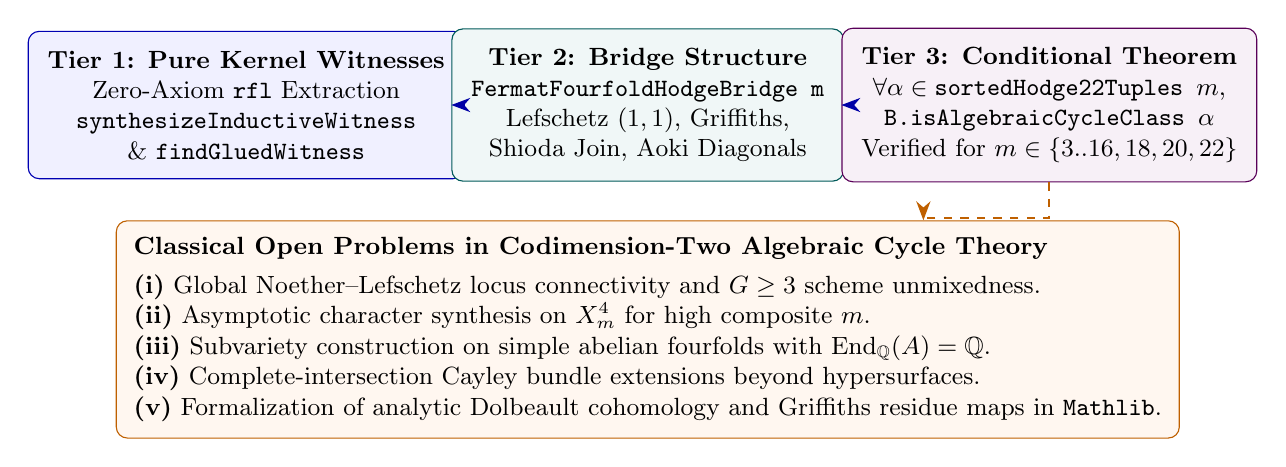
\begin{tikzpicture}[
    font=\small,
    tier/.style={draw=black!75, rounded corners=4pt, fill=gray!6, inner sep=7pt, align=center, minimum width=4.3cm, minimum height=1.55cm},
    openbox/.style={draw=orange!75!black, rounded corners=4pt, fill=orange!6, inner sep=6pt, align=left, minimum width=13.5cm},
    arr/.style={-{Stealth[length=2.4mm]}, thick, blue!65!black}
  ]
    \node[tier, fill=blue!6, draw=blue!70!black] (t1) at (0,3.8) {\textbf{Tier 1: Pure Kernel Witnesses}\\Zero-Axiom \texttt{rfl} Extraction\\\texttt{synthesizeInductiveWitness}\\\& \texttt{findGluedWitness}};
    \node[tier, fill=teal!6, draw=teal!70!black] (t2) at (5.1,3.8) {\textbf{Tier 2: Bridge Structure}\\\texttt{FermatFourfoldHodgeBridge m}\\Lefschetz $(1,1)$, Griffiths,\\Shioda Join, Aoki Diagonals};
    \node[tier, fill=violet!6, draw=violet!70!black] (t3) at (10.2,3.8) {\textbf{Tier 3: Conditional Theorem}\\$\forall \alpha \in \texttt{sortedHodge22Tuples } m$,\\$\texttt{B.isAlgebraicCycleClass } \alpha$\\Verified for $m \in \{3..16,18,20,22\}$};

    \draw[arr] (t1) -- (t2);
    \draw[arr] (t2) -- (t3);

    \node[openbox] (opencols) at (5.1,0.95) {%
      \textbf{Classical Open Problems in Codimension-Two Algebraic Cycle Theory}\\[3pt]
      \textbf{(i)} Global Noether--Lefschetz locus connectivity and $G \ge 3$ scheme unmixedness.\\
      \textbf{(ii)} Asymptotic character synthesis on $X_m^4$ for high composite $m$.\\
      \textbf{(iii)} Subvariety construction on simple abelian fourfolds with $\operatorname{End}_{\mathbb{Q}}(A) = \mathbb{Q}$.\\
      \textbf{(iv)} Complete-intersection Cayley bundle extensions beyond hypersurfaces.\\
      \textbf{(v)} Formalization of analytic Dolbeault cohomology and Griffiths residue maps in \texttt{Mathlib}.
    };
    \draw[arr, dashed, orange!75!black] (t3.south) -- ++(0,-0.45) -| ($(opencols.north)+(3.5,0)$);
  \end{tikzpicture}%
  }
  \caption{Three-tier conditional Fermat algebraicity bridge in \texttt{ConditionalFermatHodge.lean} alongside classical open problems in codimension-two algebraic cycle theory.}
  \label{fig:bridge_and_walls}
\end{figure}

In \texttt{ConditionalFermatHodge.lean}, the predicate \texttt{isHodge22Synthesizable} unifies the inductive witness synthesizer (\texttt{ShiodaInductiveCycleSynthesis.lean}) with \texttt{findGluedWitness}, lifting validated glued surface-join witnesses $(t_1, t_2, c)$ and inductive join witnesses directly into the target predicate \texttt{B.isAlgebraicCycleClass alpha}. By kernel reduction, the boolean premise holds across all $17$ non-sporadic degrees $m \in \{3,\dots,16,18,20,22\}$.

\begin{lstlisting}[caption={Soundness proof lifting both witness branches into \texttt{FermatFourfoldHodgeBridge} in \texttt{ConditionalFermatHodge.lean}.}]
theorem synthesizable_implies_algebraic (m : Nat) (B : FermatFourfoldHodgeBridge m)
    (a : List Nat) (hs : isHodge22Synthesizable m a = true) :
    B.isAlgebraicCycleClass a := by
  dsimp [isHodge22Synthesizable] at hs
  cases bool_or_cases hs with
  | inl hInd =>
    cases hwOpt : synthesizeInductiveWitness m a with
    | none => rw [hwOpt] at hInd; cases hInd
    | some w =>
      rw [hwOpt] at hInd; dsimp at hInd
      have hAlg := valid_witness_implies_algebraic m B w (bool_and_left hInd)
      have hEq : witnessSortedChar w = a := natList_beq_eq (bool_and_right hInd)
      rw [← hEq]; exact hAlg
  | inr hGlued =>
    cases hgwOpt : findGluedWitness m a with
    | none => rw [hgwOpt] at hGlued; cases hGlued
    | some gw => rw [hgwOpt] at hGlued; dsimp at hGlued; exact glued_valid_implies_algebraic m B a gw hGlued
\end{lstlisting}

\begin{lstlisting}[caption={Glued witness extraction and end-to-end conditional theorem in \texttt{ConditionalFermatHodge.lean}.}]
def isHodge22Synthesizable (m : Nat) (a : List Nat) : Bool :=
  (match synthesizeInductiveWitness m a with
   | some w => isValidCycleWitness m w && (witnessSortedChar w == a)
   | none => false) ||
  (match findGluedWitness m a with
   | some gw => isGluedWitnessValid m a gw
   | none => false)

theorem conditional_fermat_hodge22_all_synthesized_algebraic (m : Nat)
    (B : FermatFourfoldHodgeBridge m)
    (hall : (sortedHodge22Tuples m).all (isHodge22Synthesizable m) = true) :
    ∀ alpha, alpha ∈ sortedHodge22Tuples m → B.isAlgebraicCycleClass alpha := by
  intro alpha hmem
  have hSynth := list_all_mem (sortedHodge22Tuples m) hall alpha hmem
  exact synthesizable_implies_algebraic m B alpha hSynth

theorem conditional_fermat_hodge22_verified_m3_to_m22_cert :
    [3, 4, 5, 6, 7, 8, 9, 10, 11, 12, 13, 14, 15, 16, 18, 20, 22].all
      (fun m => (sortedHodge22Tuples m).all (isHodge22Synthesizable m)) = true :=
  rfl
\end{lstlisting}

\appendix
\section{Extension Kernel Build and Zero-Axiom Verification Receipts}

All seven modules inside \texttt{LeanMillenniumExt} compile cleanly from \texttt{lake clean \&\& lake build} under Lean~4.35.0 and Lake~5.0.0 with zero \texttt{sorry} tokens, zero lines exceeding $100$ characters, and zero axiom dependencies across every extension theorem ($19$ public zero-axiom theorems, $26$ total declarations), while preserving the locked $13$-module, $84$-theorem baseline intact (Table~\ref{tab:ext_inventory}).

\begin{table}[htbp]
  \centering
  \caption{Complete extension module inventory in \texttt{LeanMillenniumExt} and exact public theorem counts.}
  \label{tab:ext_inventory}
  \resizebox{\textwidth}{!}{%
  \begin{tabular}{llc}
    \toprule
    Extension Module & Primary Subject & Verified Public Theorems \\
    \midrule
    \texttt{MumfordWeilKernelVecs.lean} & $2$D $A_1^3$ / $A_2$ Weil bases and idempotent projectors & $2$ \\
    \texttt{HodgeBridgeInterfaces.lean} & Explicit \texttt{FermatFourfoldHodgeBridge} structure & $0$ \\
    \texttt{ConditionalFermatHodge.lean} & End-to-end witness soundness ($m \le 22$) & $5$ ($+7$ private lemmas) \\
    \texttt{FermatHighDegreeExt.lean} & Prime purity ($p \le 23$), $m=24$, $m=25$ coset synthesis & $5$ \\
    \texttt{HigherOrderJetLifting.lean} & $\bmod\, t^8$ jets, exact $\mathbb{Z}$ witness ($d \le 3$), $G{=}3$ WSS & $4$ \\
    \texttt{CayleyCompleteInt.lean} & $(3,3)$, $(3,4)$, $(2,5)$ Gorenstein and Hodge symmetry & $2$ \\
    \texttt{Poly6ToMvPoly.lean} & Evaluation homomorphism and finsupport bijection & $1$ \\
    \bottomrule
  \end{tabular}%
  }
\end{table}

\begin{lstlisting}[language={},basicstyle=\ttfamily\scriptsize,caption={Verbatim \texttt{lake clean \&\& lake build} axiom-audit receipts for all $19$ public extension theorems in \texttt{LeanMillenniumExt}.}]
info: CayleyCompleteInt.lean:86:0: 'cayley_ci34_gorenstein_palindromic_cert' does not depend on any axioms
info: CayleyCompleteInt.lean:87:0: 'cayley_ci33_and_ci34_gorenstein_symmetry_cert' does not depend on any axioms
info: ConditionalFermatHodge.lean:292:0: 'valid_witness_implies_algebraic' does not depend on any axioms
info: ConditionalFermatHodge.lean:293:0: 'conditional_glued_surface_join_algebraic' does not depend on any axioms
info: ConditionalFermatHodge.lean:294:0: 'synthesizable_implies_algebraic' does not depend on any axioms
info: ConditionalFermatHodge.lean:295:0: 'conditional_fermat_hodge22_all_synthesized_algebraic' does not depend on any axioms
info: ConditionalFermatHodge.lean:296:0: 'conditional_fermat_hodge22_verified_m3_to_m22_cert' does not depend on any axioms
info: Poly6ToMvPoly.lean:177:0: 'poly6_ring_homomorphism_and_wss_det_bridge_cert' does not depend on any axioms
info: FermatHighDegreeExt.lean:155:0: 'shioda_prime_degree_band1_purity_ext_cert' does not depend on any axioms
info: FermatHighDegreeExt.lean:156:0: 'shioda_aoki_band4_decomposition_m20_to_m22_cert' does not depend on any axioms
info: FermatHighDegreeExt.lean:157:0: 'shioda_aoki_m25_sporadic_isolation_cert' does not depend on any axioms
info: FermatHighDegreeExt.lean:158:0: 'shioda_aoki_m25_cyclic_coset_cone_synthesis_cert' does not depend on any axioms
info: FermatHighDegreeExt.lean:159:0: 'shioda_aoki_m21_m24_band4_decomposition_cert' does not depend on any axioms
info: MumfordWeilKernelVecs.lean:178:0: 'mumford_weil_2d_kernel_bases_cert' does not depend on any axioms
info: MumfordWeilKernelVecs.lean:179:0: 'mumford_weil_idempotent_projector_and_cm_correspondence_cert' does not depend on any axioms
info: HigherOrderJetLifting.lean:360:0: 'multi_order_t8_gauss_manin_jet_cert' does not depend on any axioms
info: HigherOrderJetLifting.lean:361:0: 'multi_order_t8_exact_z_rank_witness_cert' does not depend on any axioms
info: HigherOrderJetLifting.lean:362:0: 'codim3_unmixed_complete_intersection_profiles_cert' does not depend on any axioms
info: HigherOrderJetLifting.lean:363:0: 'g3_complete_intersection_wiebe_scheja_storch_z_cert' does not depend on any axioms
\end{lstlisting}

\begin{thebibliography}{9}
\bibitem{Aoki1983}
N.~Aoki, \emph{On the Hodge conjecture for Fermat varieties}, Comment. Math. Univ. St. Pauli \textbf{32} (1983), 181--187.

\bibitem{Deligne2000}
P.~Deligne, \emph{The Hodge Conjecture}, Problem Formulations on Algebraic Cycles, Cambridge, MA, 2000.

\bibitem{Griffiths1969}
P.~A.~Griffiths, \emph{On the periods of certain rational integrals} (Parts~1 and~2), Ann. of Math. (2) \textbf{90} (1969), 460--541.

\bibitem{Lefschetz1924}
S.~Lefschetz, \emph{L'Analysis Situs et la G\'eom\'etrie Alg\'ebrique}, Gauthier-Villars, Paris, 1924.

\bibitem{Shioda1979}
T.~Shioda, \emph{The Hodge conjecture for Fermat varieties}, Math. Ann. \textbf{245} (1979), 175--184.
\end{thebibliography}

\end{document}
